% The optional argument [<+->] means everything on the frame will be displayed incrementally.
\section{Introduction}

\begin{frame}[<+->]
  \frametitle{Goals}   
  \begin{block}{\texttt{libMesh} is not}
  \begin{itemize}
  \item {A physics implementation.}
  \item {A stand-alone application.}
  \end{itemize}
  \end{block}
  \begin{block}{\texttt{libMesh} is}
  \begin{itemize}
  \item {A software library and toolkit.}
  \item {Classes and functions for writing parallel adaptive finite
element applications.}
  \item {An interface to linear algebra, meshing, partitioning, etc.
libraries.}
  \end{itemize}
  \end{block}
\end{frame}


\begin{frame}
  %\frametitle{}
  \begin{columns}[t]
    \column{.5\textwidth}
    \begin{block}{}%A general class of PDE}      %find $u(\bv{x},t)$ such that
      For most applications we assume there is a Boundary Value Problem
      to be approximated in a Finite Element function space
      \begin{eqnarray}
	\label{eqn:general_pde}
	\nonumber
	M \dt{u} & = & F( u ) \;\;\;\; \in \Omega
        \\
	\nonumber
	G( u ) & = & 0 \;\;\;\; \in \Omega
	\\
	\nonumber
	u & = & u_D \;\; \in \partial \Omega_D
	\\
	\nonumber
	N(u) & = & 0 \;\; \in \partial \Omega_N
 	\\
 	\nonumber
 	u(\bv{x}, 0) & = & u_0(\bv{x}) 
      \end{eqnarray}
    \end{block}
    %\pause
    \column{.5\textwidth}
    %\begin{block}{}
      \begin{center}
	%\fbox{
	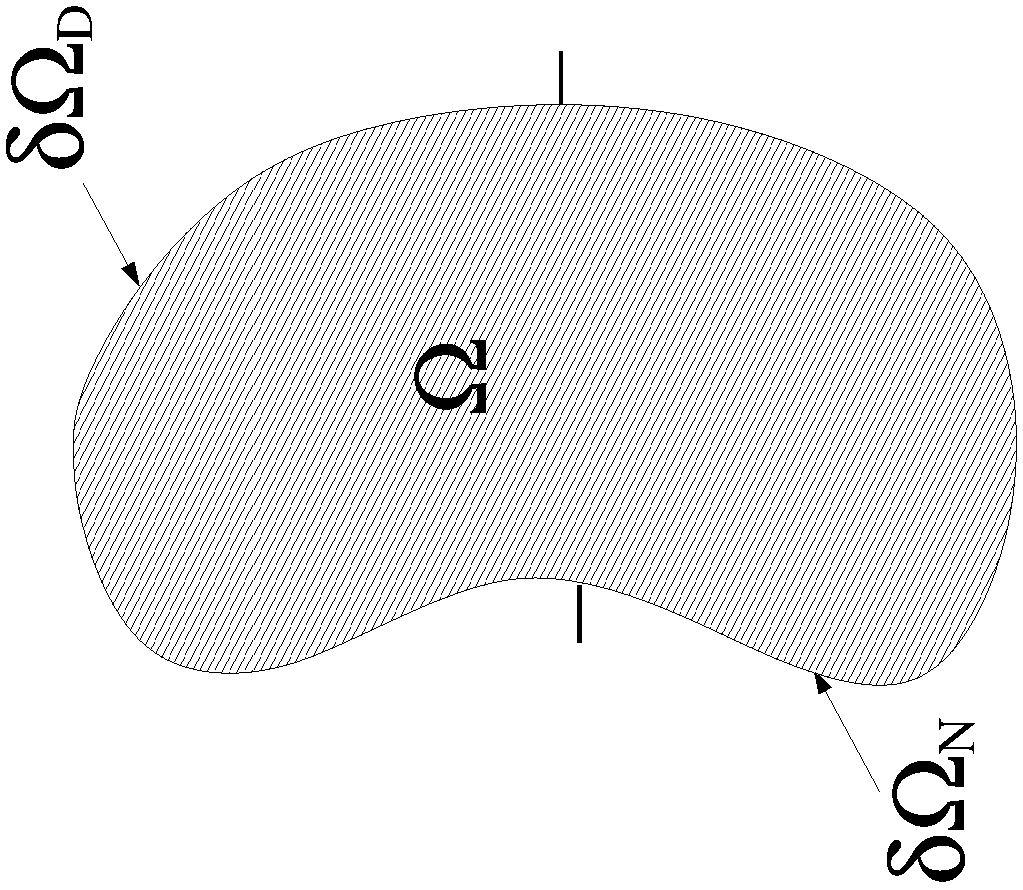
\includegraphics[width=2in,angle=-90]{figs/domain}
	%}
      \end{center}
    %\end{block}
  \end{columns}
%%  \begin{itemize}
%%    \item $\mathcal{N}( u )$ is a nonlinear operator which depends on the unknown
%%      $u$ and its spatial gradients%, $\bv{f}$ is a forcing function
%%    % \item With slight modifications, a wide range of physically interesting problems fall into this class
%%    \item Use generic numerical methods to treat many problems in the same framework
%%  \end{itemize}
\end{frame}


\begin{frame}
  %\frametitle{}
  \begin{columns}[t]
    \column{.5\textwidth}
    \begin{block}{}%A general class of PDE}
      \begin{itemize}
      \item{
	Associated to $\Omega$ is the \texttt{Mesh} data
	structure
      }
	
      \item{A \texttt{Mesh} is basically
	a collection of geometric elements and nodes}
      \end{itemize}
      \begin{equation}
	\label{eqn:discretized_domain}
	\nonumber
	\Omega^h:=\bigcup_e \Omega_e
      \end{equation}
    \end{block}
    %\pause
    \column{.5\textwidth}
    %\begin{block}{}
      \begin{center}
	%\fbox{
	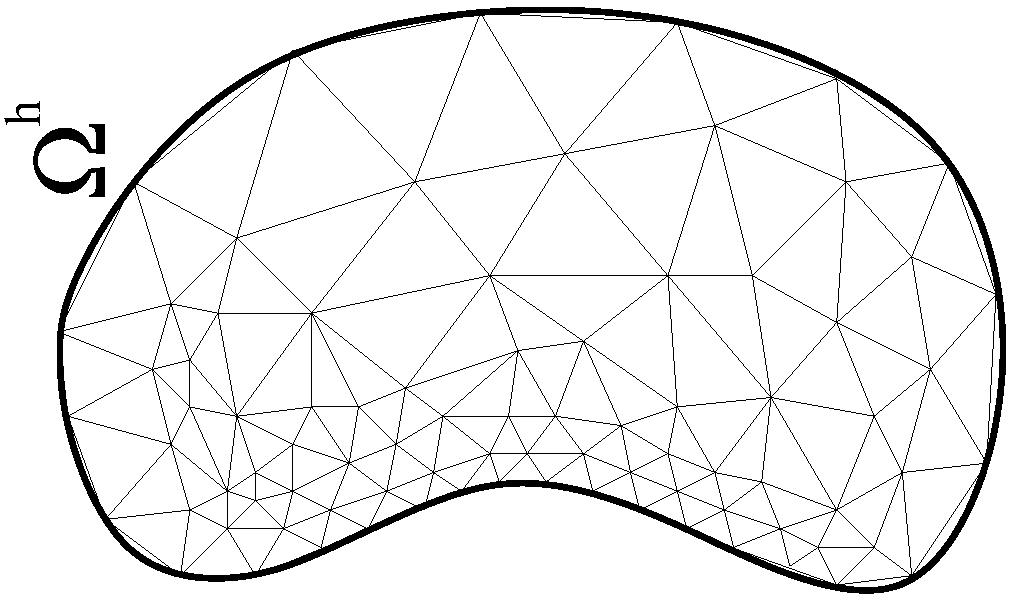
\includegraphics[width=2in,angle=-90]{figs/discretized_domain}
	%}
      \end{center}
    %\end{block}
  \end{columns}
\commentout{
  \visible<2>
  {
  \begin{itemize}
    \item{libMesh provides some simple structured mesh generation routines
      as well as an interface to Triangle.}
  \end{itemize}
  }
}
\end{frame}


%% \begin{frame}
%%   \frametitle{The Mesh}
%%   \begin{block}{}
%%     The \texttt{Mesh} data structure provides: 
%%     \begin{itemize}
%%     \item{Iterator access to the nodes and elements}
%%     \end{itemize}
%%   \end{block}
%% \end{frame}
